%\documentclass[12pt,draftcls,peerreview, onecolumn]{IEEEtran}

%\documentclass[10pt,draftcls,onecolumn]{IEEEtran}
\documentclass[10pt,conference]{IEEEtran}

%\usepackage[T1]{fontenc}
%\usepackage[latin1]{inputenc}
%\usepackage[all]{xy}
\usepackage{stackrel}
\usepackage{subfigure}
\usepackage{epsf}
\usepackage{amsmath,amssymb}
\usepackage{graphicx}
\usepackage{color}
\usepackage{cite}
\usepackage{multirow,tabularx}
\usepackage{ifthen}

% Add these after the document class declaration
\usepackage{times}
\usepackage{pgf-pie}
\input{epsf.sty}
%\pagestyle{bfheadings}
%-------------------------------

\newcommand{\showfigure}{\boolean{true}}
%\newcommand{\showfigure}{\boolean{false}}

\newcommand{\hide}[1]{\ifthenelse{\boolean{false}}{#1}{}}

%\include{../../commonHeader}
%%%%%%%%%%%%%%%%%%%%%%
% Theorems, etc.

\newtheorem{theorem}{{\bf Theorem}}
\newtheorem{lemma}{{\bf Lemma}}
\newtheorem{proposition}[theorem]{Proposition}
\newtheorem{corollary}{{\bf Corollary}}
\newtheorem{result}{{\bf Result}}

%\newenvironment{proof}[1][Proof]{\begin{trivlist}
%\item[\hskip \labelsep {\bfseries #1}]}{\end{trivlist}}

%\newtheorem{defn}{Definition}
\newenvironment{definition}[1][Definition]{\begin{trivlist}
\item[\hskip \labelsep {\bfseries #1}]}{\end{trivlist}}

\newenvironment{example}[1][Example]{\begin{trivlist}
\item[\hskip \labelsep {\bfseries #1}]}{\end{trivlist}}

\newenvironment{remark}[1][Remark]{\begin{trivlist}
\item[\hskip \labelsep {\bfseries #1}]}{\end{trivlist}}

\newcommand{\qed}{\nobreak \ifvmode \relax \else
      \ifdim\lastskip<1.5em \hskip-\lastskip
      \hskip1.5em plus0em minus0.5em \fi \nobreak
      \vrule height0.75em width0.5em depth0.25em\fi}


\newtheorem{fact}{Fact}
\newtheorem{obs}{Observation}

%%%%%%%%%%%%%%%%%%%%%%
% Environments

\newcommand{\beq}{\begin{equation}}
\newcommand{\eeq}{\end{equation}}
\newcommand{\barr}{\begin{array}}
\newcommand{\earr}{\end{array}}

\newcommand{\benum}{\begin{enumerate}}
\newcommand{\eenum}{\end{enumerate}}

\newcommand{\bit}{\begin{itemize}}
\newcommand{\eit}{\end{itemize}}

\newcommand{\bc}{\begin{center}}
\newcommand{\ec}{\end{center}}

\newcommand{\bdes}{\begin{description}}
\newcommand{\edes}{\end{description}}

\newcommand{\bfig}{\begin{figure}}
\newcommand{\efig}{\end{figure}}

\newcommand{\bemq}{\begin{quote} \begin{em}}
\newcommand{\eemq}{\end{em} \end{quote}}

\newcommand{\bmp}{\begin{minipage}}
\newcommand{\emp}{\end{minipage}}


%%%%%%%%%%%%%%%%%%%%%%
% References

\newcommand{\eqn}[1]{(\ref{#1})}
\newcommand{\fgr}[1]{Fig.~\ref{#1}}
\newcommand{\tbl}[1]{Table~\ref{#1}}
\newcommand{\secref}[1]{Section~\ref{#1}}
\newcommand{\apndx}[1]{Appendix~\ref{#1}}
\newcommand{\app}[1]{Appendix~\ref{#1}}
\newcommand{\chpref}[1]{Chapter~\ref{#1}}
\newcommand{\lemref}[1]{Lemma~\ref{#1}}
\newcommand{\thmref}[1]{Theorem~\ref{#1}}

%%%%%%%%%%%%%%%%%%%%%%
% Brackets

\newcommand{\brac}[1]{\left({#1}\right)}
\newcommand{\sbrac}[1]{\left[{#1}\right]}
\newcommand{\cbrac}[1]{\left\{{#1}\right\}}

\newcommand{\floor}[1]{\left\lfloor{#1}\right\rfloor}

%%%%%%%%%%%%%%%%%%%%%%
% Misc

\newcommand{\expc}[2][]{E^{#1}\left[{#2}\right]}

\newcommand{\set}[1]{\{#1\}}

\newcommand{\ul}{\underline}
\newcommand{\smq}[1]{{\it #1}}
\newcommand{\ave}[1]{\overline{#1}}

\newcommand{\recip}[1]{\frac{1}{{#1}}}

%%%%%%%%%%%%%%%%%%%%%%
% Indicator function

\newcommand{\indic}[1]{I\left[{#1}\right]}

%%%%%%%%%%%%%%%%%%%%%%
% Superscripts
\newcommand{\supth}{^{{\mathrm{th}}}}
\newcommand{\kth}{^{{\mathrm{th}}}}
\newcommand{\supnd}{^{{\mathrm{nd}}}}
\newcommand{\suprd}{^{{\mathrm{rd}}}}

\newcommand{\given}{\arrowvert}

%%%%%%%%%%%%%%%%%%%%%%
% Symbols

\newcommand{\db}{{\mathrm dB}}
\newcommand{\Om}{\hat{\Omega}}

\newcommand{\define}{\triangleq}
%\newcommand{\define}{\stackrel{\triangle}{=}}
%\newcommand{\implies}{\Rightarrow}
%\newcommand{\tendsto}{\rightarrow}
\newcommand{\tendsto}{\to}

\newcommand{\degree}{^{\circ}}
\newcommand{\kroneck}{\otimes}

%%%%%%%%%%%%%%%%%%%%%%
% Special phrases

\newcommand{\ie}{{\it i.e.}}
\newcommand{\eg}{{\it e.g.}}
\newcommand{\etal}{{\it et al.}}
\newcommand{\wrt}{w.r.t.}
\newcommand{\vs}{{\it vs.}}
\newcommand{\viz}{{\it viz. }}

%%%%%%%%%%%%%%%%%%%%%%
% Matrix related

\newcommand{\tvec}{\text{vec}} % \vec is already defined
\newcommand{\mtx}[1]{{\bf #1}} % matrix
\newcommand{\mtxg}[1]{{\boldsymbol #1}} % matrix for greek symbol

\newcommand{\trp}{\text{T}} % transpose
\newcommand{\trc}[1]{\text{Tr}\left\{{#1}\right\}} % trace

%%%%%%%%%%%%%%%%%%%%%%
% Special matrices

\newcommand{\mi}[1]{\mtx{I}_{#1}}
\newcommand{\mzero}{\mtx{0}}

%%%%%%%%%%%%%%%%%%%%%%
% Principal sub-matrix

\newcommand{\princ}[2]{{#2}^{({#1})}}
\newcommand{\princsup}[3]{{{#2}^{({#1})^{#3}}}}

%%%%%%%%%%%%%%%%%%%%%%
% Probability related

\newcommand{\iid}{{i.i.d.}}

\newcommand{\EX}{\mathbb{E}} % expectation operator
\newcommand{\expect}[1]{{\bf E}\left[{#1}\right]}
\newcommand{\expectpow}[2]{{\bf E}^{#2}\left[{#1}\right]}
\newcommand{\prob}[1]{\text{Pr}\brac{#1}}
\newcommand{\pr}{{\cal P}}

%%%%%%%%%%%%%%%%%%%%%%
% Derivatives

\newcommand{\deriv}[2]{\frac{d{#1}}{d{#2}}}
\newcommand{\pderiv}[2]{\frac{\partial{#1}}{\partial{#2}}}

%%%%%%%%%%%%%%%%%%%%%%
% Slides

\newcommand{\bsp}{\begin{slide*}}
\newcommand{\esp}{\end{slide*}}
\newcommand{\bsl}{\begin{slide}}
\newcommand{\esl}{\end{slide}}
\newcommand{\vsp}[1]{\vspace{#1}}

%%%%%%%%%%%%%%%%%%%%%%%%
% Theorem
\newcommand{\blem}{\begin{lemma}}
\newcommand{\elem}{\end{lemma}}
\newcommand{\bthm}{\begin{theorem}}
\newcommand{\ethm}{\end{theorem}}

%-------------------------------
% This paper's specific

\newcommand{\nbm}[1]{{[\bf nbm: #1]}}
\newcommand{\parag}[1]{[\textsl{Parag: #1}]}

\newcommand{\EHS}{\text{EH}}
\newcommand{\nonEHS}{\textsl{nonEH}}

\newcommand{\Pehs}{\bar{P}_{\EHS}}
\newcommand{\RoptNonEHS}{\bar{R}^{\ast}_{\nonEHS}}
\newcommand{\RiioptNonEHS}{\bar{R}^{'\ast}_\text{i}}
\newcommand{\RioptNonEHS}{\bar{R}^{\ast}_\text{i}}
\newcommand{\RoptEHS}{\bar{R}^{\ast}_{\EHS}}

\newcommand{\Rtwo}{R_{\EHS}(\Pehs - \delta,i)}
\newcommand{\Rone}{R_{\nonEHS}(\Pehs - \delta,i)}
\newcommand{\Pmax}{\bar{P}_{\max}}

\newcommand{\Preq}{P_\textsl{req}}
\newcommand{\Ptr}{P_\textsl{tx}}

\newcommand{\asg}{\stackrel{as}{>}}
\newcommand{\asl}{\stackrel{as}{<}}
\newcommand{\aseq}{\stackrel{as}{=}}

\IEEEoverridecommandlockouts

\begin{document}

\title{Probabilistic Analysis of the Squash Sport}
%
\author{Prathamesh D. Anwekar and Kaushal S. Kirpekar
\thanks{The authors are students of the Dept.\ of Electrical and Electronics
     Eng.\ at the Birla Institute of Technology and Science (BITS), Pilani,
     India.}
%
\thanks{Emails: f20201039@pilani.bits-pilani.ac.in,
     f20200828@pilani.bits-pilani.ac.in}
}

\IEEEaftertitletext{\vspace{-0.5\baselineskip}}

\maketitle
\newcommand{\ceil}[1]{\lceil{#1}\rceil}


\begin{abstract}
The research question for this study is: what is the distribution of different types of shots from different areas of the court in squash, and how do these patterns vary among professional and amateur players? To answer this question, we collected data on the types and locations of shots taken by professional and amateur players during games of squash. We then used probabilistic analysis to study the distribution of these shots and to compare the strategies used by different levels of players.

Our key findings indicate that professional players tend to use a wider variety of shots and are more strategic in their shot selection than amateur players. Professional players also tend to hit more shots from the back of the court, which allows them to control the pace of the game and to set up more difficult shots for their opponents. In contrast, amateur players tend to hit more shots from the middle of the court, which can lead to more errors and a less controlled game.

The implications of these findings are significant for players, coaches, and fans of squash. By understanding the strategies used by professional players, players at all levels can learn how to improve their own game and become more competitive. Coaches can also use these findings to develop more effective training programs and strategies for their players. Finally, fans of squash can gain a greater appreciation for the skill and strategy involved in the game, and can better understand the strategies used by the top players in the sport.
\end{abstract}

\section{Introduction}
\label{sec:intro}

The game of squash is a high-intensity sport that requires a combination of physical fitness, mental agility, and strategic thinking. It is a popular and competitive sport that is played by millions of people around the world. In recent years, there has been an increasing interest in understanding the different strategies and techniques that players use to succeed in squash.

One way to analyze the strategies used in squash is through the use of probabilistic analysis. Probabilistic analysis is a statistical method that uses probability theory to study the likelihood of different events occurring. In the context of squash, probabilistic analysis can be used to study the distribution of different types of shots from different areas of the court. This can provide valuable insights into the strategies that players use, and can also be used to improve the performance of players at all levels of the game.

The purpose of this research paper is to conduct a probabilistic analysis of squash, with a focus on the distribution of different types of shots from different areas of the court. Using probabilistic analysis, we seek to identify the key factors that affect the outcome of squash matches, such as player skill, court conditions, and strategic choices. The data for this study will be collected from games played by both professional and amateur players. This will allow us to compare the strategies used by different levels of players and to see how these strategies may vary based on the level of the player.

The research paper is organized into four main sections. In the first section, we will provide a brief overview of the game of squash and its key features. In the second section, we will discuss the framework for the analysis and how the court and shots have been divided. In the third section, we will discuss the probabilistic analysis performed on the shot type, and in the fourth section, we will present the results of our probabilistic analysis on the shot outcome. In the fifth and final section, we will discuss the final conclusions of our findings for the game of squash and for players at the two levels of the game.

Our analysis is based on a data-set created by us of real-world squash matches, which we have collected and analyzed in order to extract relevant information. We use a variety of statistical and computational techniques to perform our analysis, and we present our findings in the following sections of this paper. Overall, this research paper provides a unique and valuable perspective on the game of squash, and will be of interest to players, coaches, and fans of the sport.

Given the highly dynamic nature of sports, we needed to make some assumptions which have been listed below:
\begin{enumerate}
    \item The shots leading to let or stroke were not counted for analysis.
    \item The service shots were not counted for analysis.
    \item The volley shots were not considered as a separate type.
    \item All players are assumed to be right handed. (Data has been collected for matched played by right handed players only)
    \item Each shot is assumed to be identical to another shot of the same type type, delivered from the same region.
\end{enumerate}
\section{Understanding the Court and Different Shots}
\label{sec:model}


 For better understanding and easier analysis of the data, the squash court has been divided into different regions and the different shots of both Forehand and Backhand type have been classified into different types.

\subsection{Studying the Court}
\begin{figure}[h!]
\centering
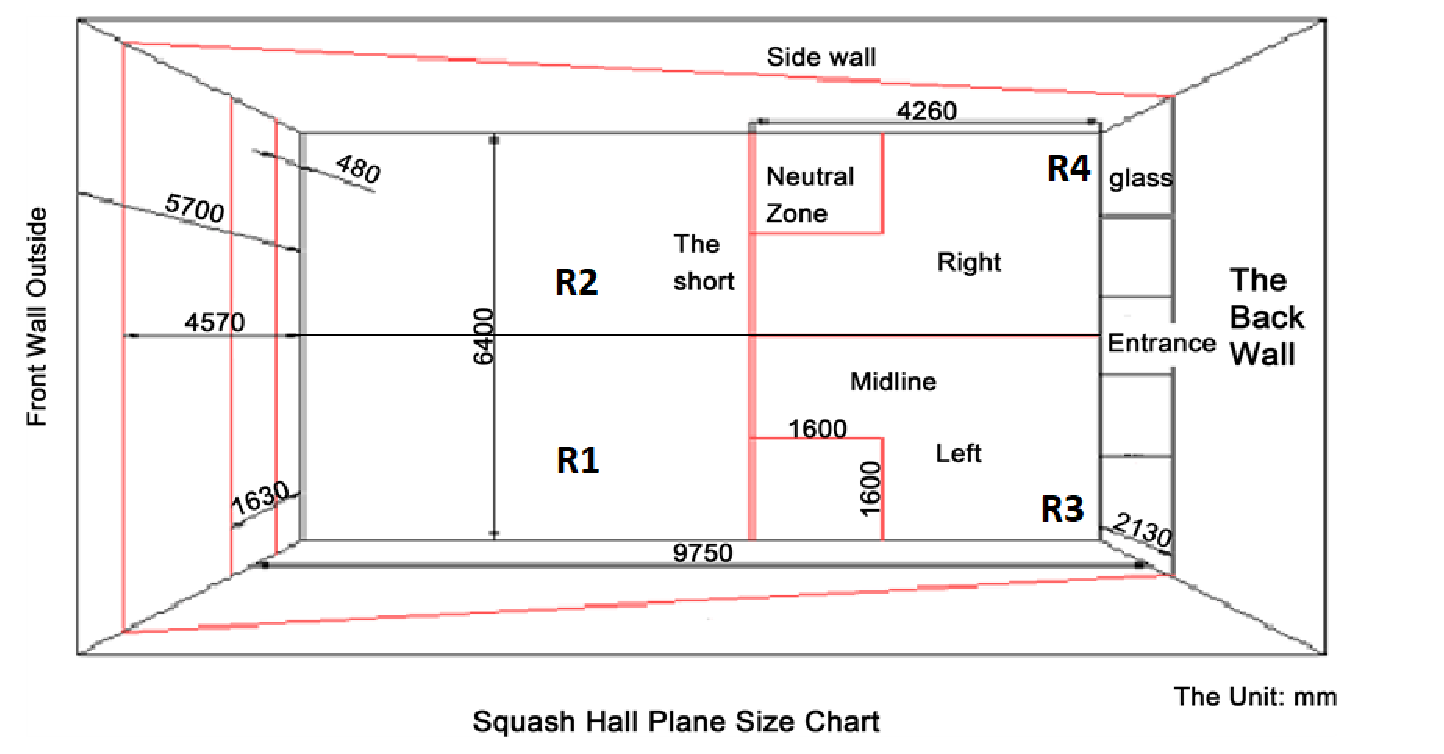
\includegraphics[height=1.5in]{SOP_SQUASH_COURT}
\caption{Dimensions and Demarcation of the Squash Court}
\label{fig:squash_court}
\end{figure}
A traditional squash court is 9.75 metres long and 6.4 metres wide. The height varies from 4.75 metres to 2.13 metres as one walks from the front wall to the back wall. 
The lower portion of 430 centimetres of the front wall is covered by tin, which is considered as an illegal region for the ball to make contact with. Going upwards, the service line is located at a height of 1.78 metres from  the ground. If the ball makes contact with the front wall beyond the out line at a height of 4.75 metres, it is considered out of play.
For analysis purposes, the court has been divided into four regions as show above in the figure 1.

\subsection{Classification of Types of Shots}

Depending on the technique used to deliver the shot, and trajectory of the ball, shots have been classified into 12 different types. These are:
\begin{enumerate}
    \item Forehand Parallel Drive 
    \item Forehand Cross Drive 
    \item Forehand Lob 
    \item Forehand Boast 
    \item Forehand Back-wall
    \item Forehand Drop
    \item Backhand Parallel Drive
    \item Backhand Cross Drive
    \item Backhand Lob
    \item Backhand Boast 
    \item Backhand Back-wall 
    \item Backhand Drop
\end{enumerate}
The outcome as a result of each shot has been classified into three types. These are:
\begin{enumerate}
    \item Normal Shot (N)
    \item Winner (W)
    \item Forced Error (F)
    \item Unforced Error (U)
\end{enumerate}

\section{Probabilistic Analysis Of Shot Type}
\label{sec:sim_res}
For the analysis, a JAVA program was written and run to get an output, for the four different regions.\\ The first number ranging from 1-12, depicts the region in which the shot was played, followed by a letter demonstrating the outcome of the shot, and every single combination has its own count.[5]
\\Figure 2 shows the analysis for one professional match. 
\begin{figure}[h!]
\centering
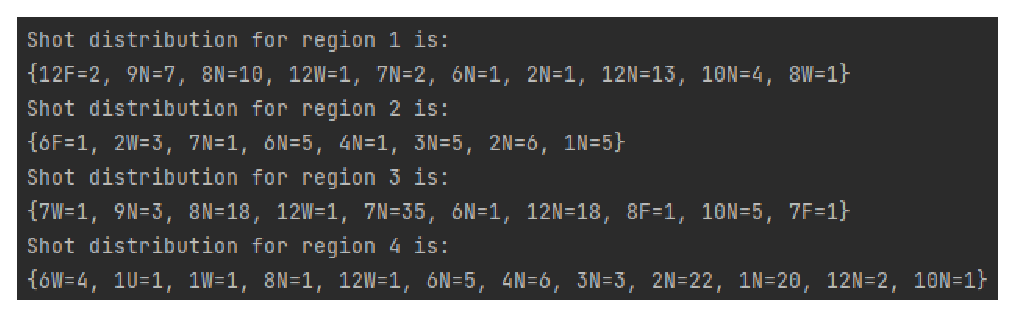
\includegraphics[height=1.0in]{analysis.eps}
\caption{Output of Java program for a Single Match Analysis}
\label{fig:java_snip}
\end{figure}

\subsection{Region-wise shot distribution for professional players}
The following tables (Tables 1-4) demonstrate different types of shots played by professional players in each of the four regions, and whether it was a successful shot or not. A total of 900 shots were analysed, across four matches.
\begin{table}[h!]
\centering
\begin{tabular}{||c c c||} 
 \hline
 Shot Type & Successful Shots & Unsuccessful Shots \\ [0.5ex]
 \hline\hline
 Backhand Parallel & 14 & 0  \\ 
 Backhand Cross & 32 & 1  \\
 Backhand Drop & 41 & 6  \\
 Backhand Lob & 22 & 1  \\
 Other & 3 & 1  \\ [1ex] 
 \hline
\end{tabular}
\caption{Different Types of Shots For Region-1}
\end{table}

\begin{table}[h!]
\centering
\begin{tabular}{||c c c||} 
 \hline
 Shot Type & Successful Shots & Unsuccessful Shots \\ [0.5ex]
 \hline\hline
 Forehand Parallel & 9 & 0  \\ 
 Forehand Cross & 30 & 1  \\
 Forehand Drop & 13 & 2  \\
 Forehand Lob & 8 & 0  \\
 Other & 6 & 0  \\ [1ex] 
 \hline
\end{tabular}
\caption{Different Types of Shots for Region-2}
\label{table:2}
\end{table}
\begin{table}[h!]
\centering
\begin{tabular}{||c c c||} 
 \hline
 Shot Type & Successful Shots & Unsuccessful Shots \\ [0.5ex]
 \hline\hline
 Backhand Parallel & 323 & 2  \\ 
 Backhand Cross & 80 & 1  \\
 Backhand Drop & 77 & 4  \\
 Backhand Boast & 19 & 1  \\
 Other & 12 & 0  \\ [1ex] 
 \hline
\end{tabular}
\caption{Different Types of Shots for Region-3}
\label{table:2}
\end{table}

\begin{table}[h!]
\centering
\begin{tabular}{||c c c||} 
 \hline
 Shot Type & Successful Shots & Unsuccessful Shots \\ [0.5ex]
 \hline\hline
 Forehand Parallel & 97 & 2  \\ 
 Forehand Cross & 98 & 1  \\
 Forehand Drop & 26 & 1  \\
 Forehand Boast & 19 & 2  \\
 Other & 17 & 1  \\ [1ex] 
 \hline
\end{tabular}
\caption{Different Types of Shots for Region-4}
\label{table:2}
\end{table}

\subsection{Region-wise shot distribution for intermediate players}
The following tables (Tables 5-8) demonstrate different types of shots played by intermediate players in each of the four regions, and whether it was a successful shot or not.  A total of 500 shots were analysed, across four matches.
\begin{table}[h!]
\centering
\begin{tabular}{||c c c||} 
 \hline
 Shot Type & Successful Shots & Unsuccessful Shots \\ [0.5ex]
 \hline\hline
 Backhand Parallel & 5 & 1  \\ 
 Backhand Cross & 10 & 2  \\
 Backhand Drop & 12 & 5  \\
 Backhand Lob & 3 & 1  \\
 Other & 5 & 1  \\ [1ex] 
 \hline
\end{tabular}
\caption{Different Types of Shots For Region-1}
\label{table:1}
\end{table}

\begin{table}[h!]
\centering
\begin{tabular}{||c c c||}
 \hline
 Shot Type & Successful Shots & Unsuccessful Shots \\ [0.5ex]
 \hline\hline
 Forehand Parallel & 14 & 3  \\ 
 Forehand Cross & 11 & 1  \\
 Forehand Drop & 12 & 2  \\
 Forehand Lob & 12 & 2  \\
 Other & 4 & 0  \\ [1ex] 
 \hline
\end{tabular}
\caption{Different Types of Shots for Region-2}

\end{table}

\begin{table}[h!]
\centering
\begin{tabular}{||c c c||} 
 \hline
 Shot Type & Successful Shots & Unsuccessful Shots \\ [0.5ex]
 \hline\hline
 Backhand Parallel & 108 & 11  \\ 
 Backhand Cross & 52 & 2  \\
 Backhand Drop & 23 & 4  \\
 Backhand Boast & 9 & 1  \\
 Other & 6 & 2  \\ [1ex] 
 \hline
\end{tabular}
\caption{Different Types of Shots for Region-3}

\end{table}
\begin{table}[h!]
\centering
\begin{tabular}{||c c c||} 
 \hline
 Shot Type & Successful Shots & Unsuccessful Shots \\ [0.5ex]
 \hline\hline
 Forehand Parallel & 71 & 4  \\ 
 Forehand Cross & 42 & 1  \\
 Forehand Drop & 8 & 1  \\
 Forehand Boast & 18 & 2  \\
 Other & 7 & 1  \\ [1ex] 
 \hline
\end{tabular}
\caption{Different Types of Shots for Region-4}
\end{table}

\subsection{Shot Outcome for Professional Level Matches}
The shot outcome was analysed for professional matches and the following chart shows the distribution of the point outcome in the form of winner, forced error or unforced error, in percentages.
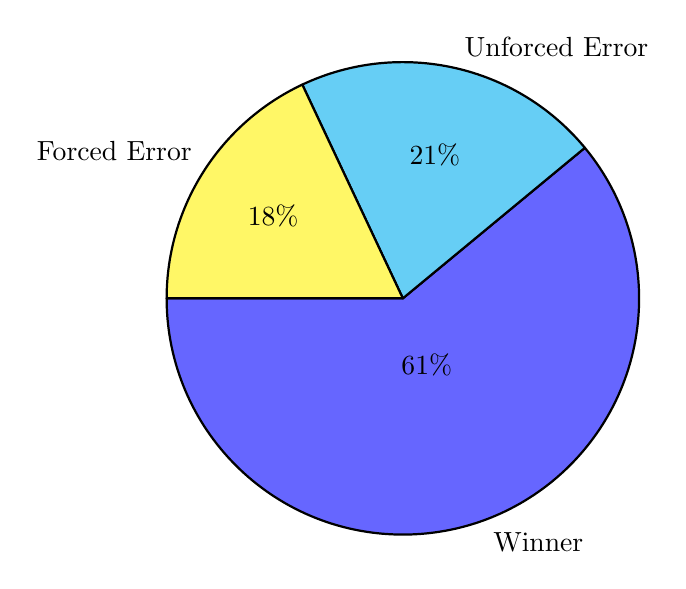
\begin{tikzpicture}
\pie [rotate = 180] {61/Winner, 21/Unforced Error , 18/Forced Error }
\end{tikzpicture}

\subsection{Shot Outcome for Intermediate Level Matches}
The shot outcome was analysed for intermediate matches and the following chart shows the distribution of the point outcome in the form of winner, forced error or unforced error, in percentages.
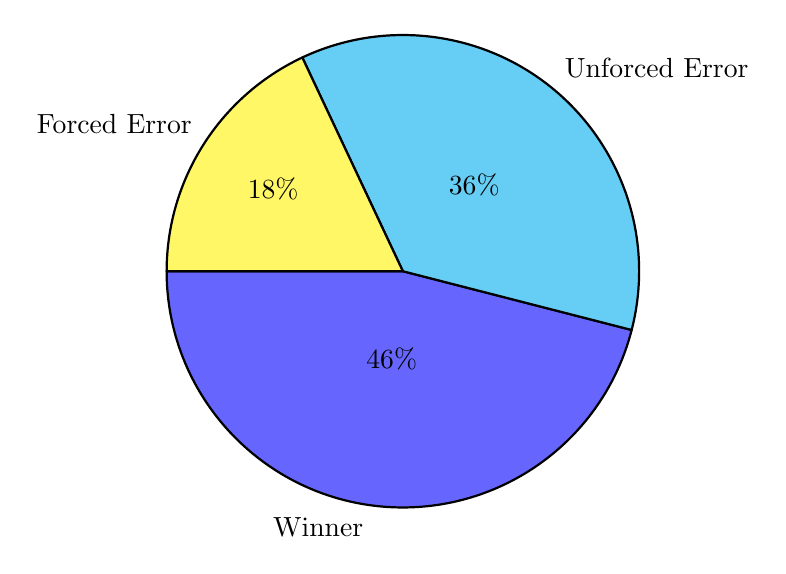
\begin{tikzpicture}
\pie [rotate = 180] {46/Winner, 36/Unforced Error , 18/Forced Error }
\end{tikzpicture}


\section{Probabilistic Analysis Of Shot Output}
\label{sec:Probabilistic Analysis}

\subsection{Winner Shot Analysis}
At the professional level, most winners were produced from the Backhand Drop shot (40\%), followed by the Forehand Drop Shot (24\%).
\\At the intermediate level, most winners were produced from the Forehand parallel Shot (58\%).
\\This is a stark difference between the professionals and intermediates because when compared in terms of skills required, to perform a drop shot demands much higher accuracy and skill compared to a forehand parallel shot.

\subsection{Forced Error Shot Analysis}
At the professional level, most forced errors were produced from the Backhand Drop shot (42\%), followed by the Backhand Boast Shot (17\%).
\\At the intermediate level, most forced errors were produced from the Backhand parallel Shot (34\%).

\subsection{Unforced Error Shot Analysis}
At the professional level, most unforced errors were produced from the Backhand Drop shot (53\%), followed by the Forehand Boast Shot (15\%).
\\At the intermediate level, most forced errors were produced from the Backhand drop Shot (40\%).
\\This is indicative of the mistakes both professionals and intermediates make. Both make the most unforced errors while trying to get the Backhand Drop right.

\section{Conclusions}
The following conclusions are drawn from the entire analysis:
\begin{enumerate}
\item At the professional level, 61 percentage of points are won by winners from either player, whereas at the intermediate level, this percentage is 46.
\item At the professional level, 21 percentage of points are won as a result of unforced error from either player, whereas at the intermediate level, this percentage is 36, showing the difference in quality between the two.
\item From the shot analysis, it can be seen that most of the match at the both the professional and intermediate level takes place in the rear part of the court, which is down to the reason that this adds more control to the game. Moreover, the backhand rear side of the court is the region that is most operated by the players, playing the Backhand Parallel shot with utmost skill to keep the ball moving.
\item From the probabilistic analysis, it can be seen that at both the professional and intermediate level, the shot that produces unforced errors is the Backhand Drop shot, but the upside of this shot is very high as it also produces the most winners at the professional level. Hence, this is a shot that every player should focus on mastering. 
\item It is also observed that the back-wall shots are only played at the rear end of the court, and similarly the lob shots are mainly played in the front regions of the court.
\end{enumerate}



\bibliographystyle{ieeetr}
% Do not delete the \bibliography line. Just comment it out.
%\bibliography{../../Bibtex/bibJournalList,../../Bibtex/MIMO,../../Bibtex/book,../../Bibtex/standard,../../Bibtex/parag}

%\hide{
\begin{thebibliography}{10}

\bibitem{basketball_sop_referencepaper}
Mathematical Modeling and Success Probability Analysis of Basketball Shots
Kaivalya Dabhadkar, Adeesh Bhargava, and Sainath Bitragunta

\bibitem{reference_paper2}
Williams, Benjamin \& Bourdon, Pitre \& Graham-Smith, Philip \& Sinclair, Peter. (2015). A quantitative analysis of squash shot accuracy. 

\bibitem{reference_paper3}
Low, Jeff \& Sankaravel, Mohansundar \& mohd rasyid, Nelfianty \& Tengah, R.Y.. (2017). Performance analysis of the Malaysian elite youth squash players. Journal of Fundamental and Applied Sciences. 2017. 9-1074. 10.4314/jfas.v9i6s.79. 

\bibitem{squash_rules}
https://www.kreedon.com/squash-rules-game-basics-history-competitions/

\bibitem{github_repository}
https://github.com/PrathameshAnwekar/SOP-SquashProbabilisticAnalysis : Data and code

\bibitem{squash_court_diagram}
https://html.scirp.org/file/4-1730627x2.png

\bibitem{squash_court_dimensions}
https://sportspages.in/squash/squash-court-dimensions/

\end{thebibliography}
%}
\end{document}


